\section{Mục tiêu và tổ chức thực nghiệm}
Bài thực hành xây dựng ba module chia khối, DCT và lượng tử hóa để mô phỏng nén ảnh xám. Mã Zigzag, RLE, Huffman, giải mã, giải lượng tử, IDCT và ghép khối được dùng từ phần A của đề bài, giữ nguyên thuật toán. Kết quả gồm ảnh dựng lại, sai số MSE, độ dài chuỗi bit Huffman và tỉ lệ hệ số bằng 0.

Ảnh đầu vào: RaceHorses\_416x240\_frame001.png, đọc ở chế độ xám uint8. Trong báo cáo, kích thước luôn viết theo H × W: 240 × 416. Khối mẫu là khối số 0 ở góc trên bên trái. Ảnh kiểm tra đệm là vùng image[:13, :19].

\begin{center}
\small\renewcommand{\arraystretch}{1.3}
\begin{tabular}{|p{7.10cm}|p{7.10cm}|}\hline
\textbf{Thành phần} & \textbf{Nội dung} \\ \hline
cau1\_chia\_khoi.py & split\_blocks; đọc ảnh, lưới khối, thử đệm \\ \hline
cau2\_dct.py & dct\_blocks; dịch mức và biểu diễn DCT \\ \hline
cau3\_luong\_tu\_hoa.py & quantize; chạy 3 mức, lưu ảnh và CSV \\ \hline
jpeg\_support.py & Mã hỗ trợ cho sẵn trong đề bài \\ \hline
\end{tabular}
\end{center}
Môi trường thực nghiệm: Python 3.11.9, NumPy 2.4.6, OpenCV 4.14.0. Chạy cả ba chương trình với tùy chọn --no-show; số liệu được đọc trực tiếp từ CSV kết quả.

\section{Câu 1 – Chia ảnh thành khối 8×8}
Với ảnh H × W, số hàng cần đệm là (-H) mod 8 và số cột cần đệm là (-W) mod 8. Dùng np.pad với mode="edge" để sao chép điểm ảnh biên xuống phía dưới và sang phải. Sắp xếp reshape → transpose → reshape tạo các khối theo thứ tự từ trái sang phải, từ trên xuống dưới.

\begin{center}
\small\renewcommand{\arraystretch}{1.3}
\begin{tabular}{|p{2.54cm}|p{2.54cm}|p{2.54cm}|p{2.54cm}|p{2.54cm}|}\hline
\textbf{Ảnh} & \textbf{Trước đệm H × W} & \textbf{Sau đệm H × W} & \textbf{Số khối} & \textbf{blocks.shape} \\ \hline
Đầy đủ & 240 × 416 & 240 × 416 & 1.560 & (1560, 8, 8) \\ \hline
Cắt & 13 × 19 & 16 × 24 & 6 & (6, 8, 8) \\ \hline
\end{tabular}
\end{center}
Ảnh đầy đủ chia hết cho 8 nên không cần đệm. Ảnh cắt thêm 3 hàng và 5 cột; vùng đệm không được tính vào MSE sau khi ảnh giải mã được cắt về 13 × 19.

\begin{figure}[!htbp]
\centering
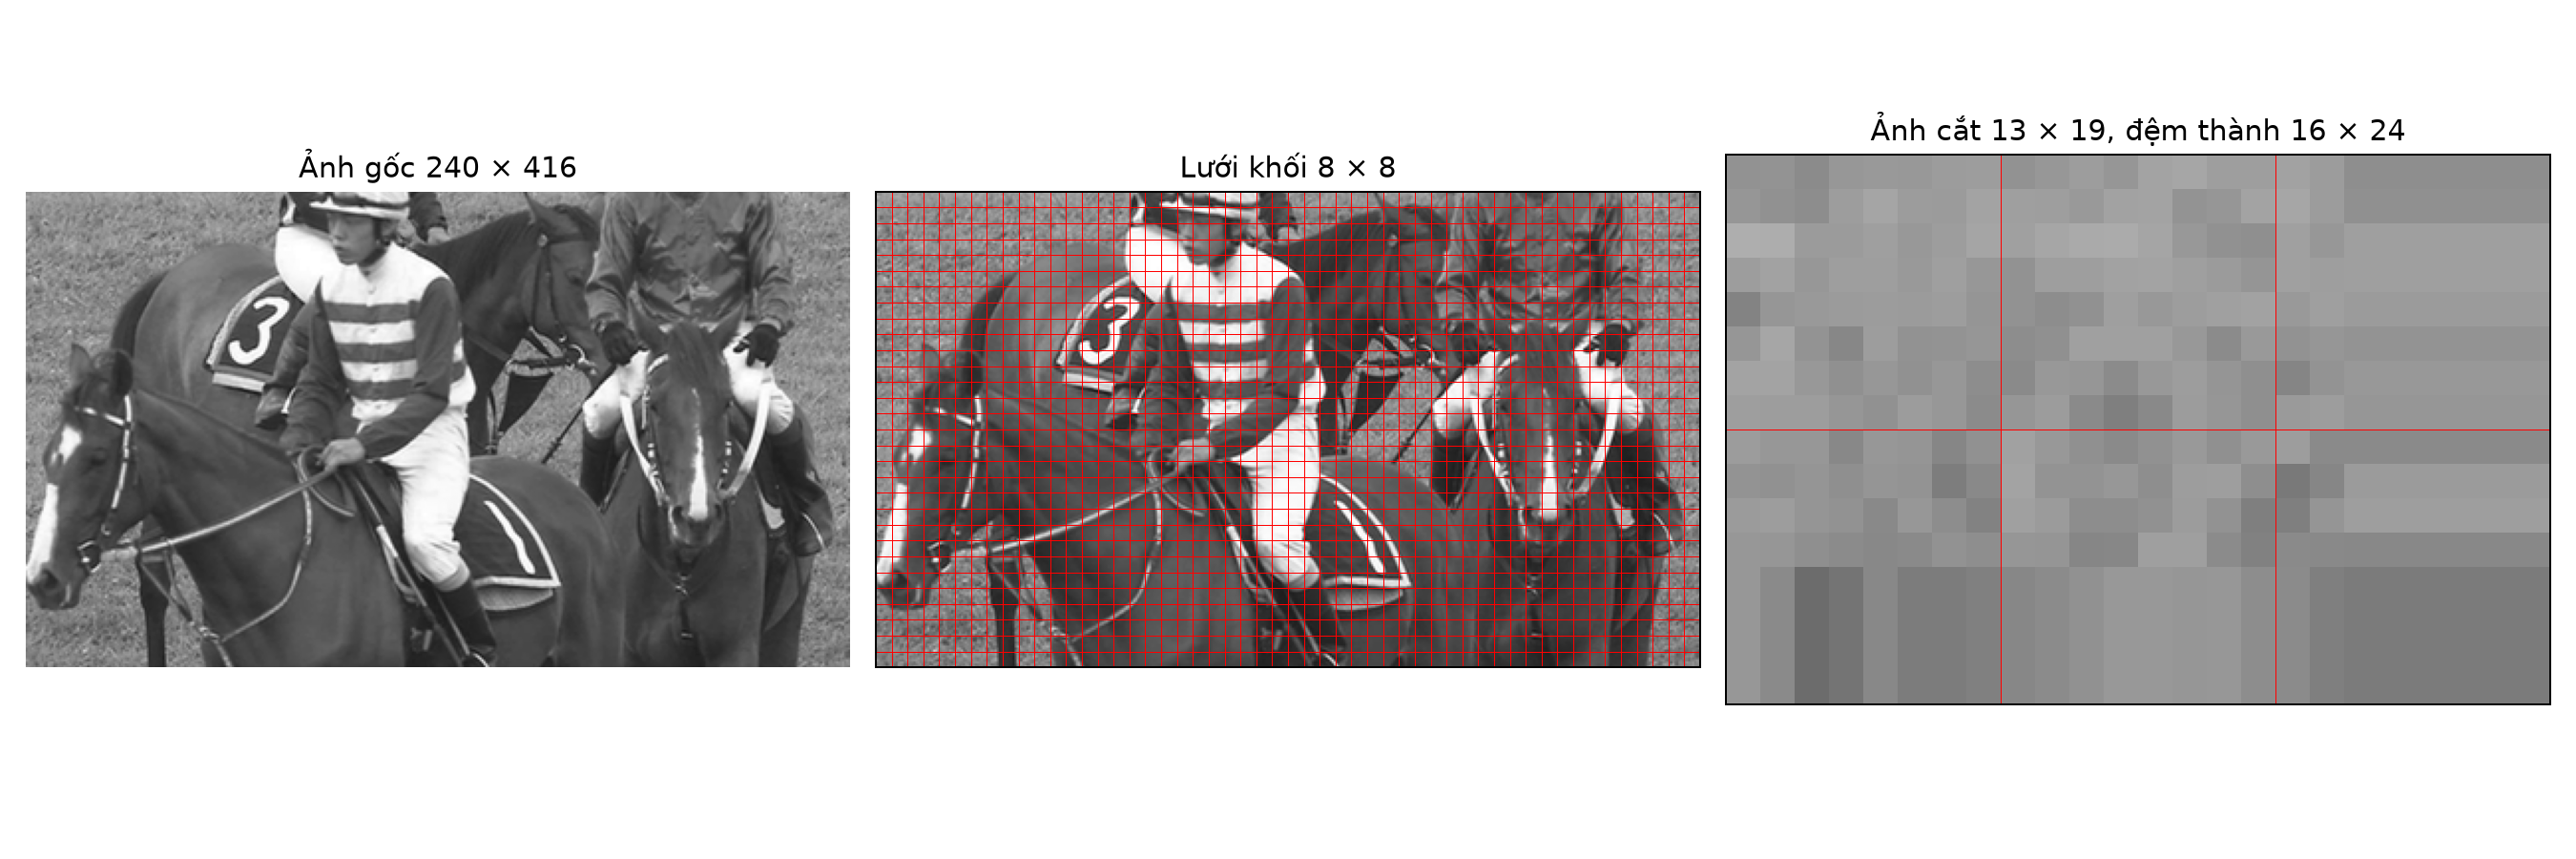
\includegraphics[width=\linewidth]{../code/ket_qua/cau1/chia_khoi.png}
\caption{Ảnh gốc, lưới khối 8×8 và ảnh cắt sau đệm.}
\end{figure}
\FloatBarrier
\subsection{Ma trận khối mẫu}
\begin{Verbatim}[fontsize=\scriptsize]
     146      148      139      151      153      152      156      157
     150      145      141      157      165      156      155      163
     174      173      155      155      159      152      157      165
     157      162      151      158      158      153      159      151
     132      150      153      155      156      155      157      149
     150      166      148      135      157      146      148      150
     163      163      152      144      151      145      151      141
     158      157      157      150      145      156      151      139
\end{Verbatim}
\clearpage
\section{Câu 2 – Biến đổi DCT}
Mỗi khối được chuyển từ uint8 sang float32 trước khi trừ 128 để tránh tràn số. Sau đó cv2.dct tính DCT hai chiều trực chuẩn. Kết quả có kích thước (N, 8, 8), kiểu float32. Dịch mức đưa miền [0, 255] về [-128, 127].

Hệ số DC nằm ở (0, 0): F[0,0] = 8 × (trung bình khối − 128). Khối mẫu có trung bình 153,171875 nên DC = 201,375. Các hệ số AC còn lại mô tả biến thiên theo tần số dọc u và ngang v; chỉ số càng lớn tương ứng dao động càng nhanh.

\subsection{Ma trận DCT của khối mẫu}
\begin{Verbatim}[fontsize=\scriptsize]
  201.38     3.80     5.23     8.29    -1.88   -10.12   -14.48     1.54
   11.61   -22.75     0.11    -1.30    18.36    -0.18    -2.98    -5.21
   -9.94     0.81     3.86     6.09     2.90     6.03     5.98    -2.21
  -22.10   -14.33    -5.98    -2.37    -3.41    -8.19    -3.77     3.70
   -7.62    -9.61   -14.07    -3.61    -8.38    11.09     1.63    -5.97
    4.38    15.98    12.44     3.32    -0.31     1.01    -5.48     1.42
    5.07     8.91    12.23    -0.96    -3.77    -7.78     0.14     0.12
    3.41     1.30     0.09    -4.57    -2.61     3.52     1.08    -0.88
\end{Verbatim}
\begin{figure}[!htbp]
\centering
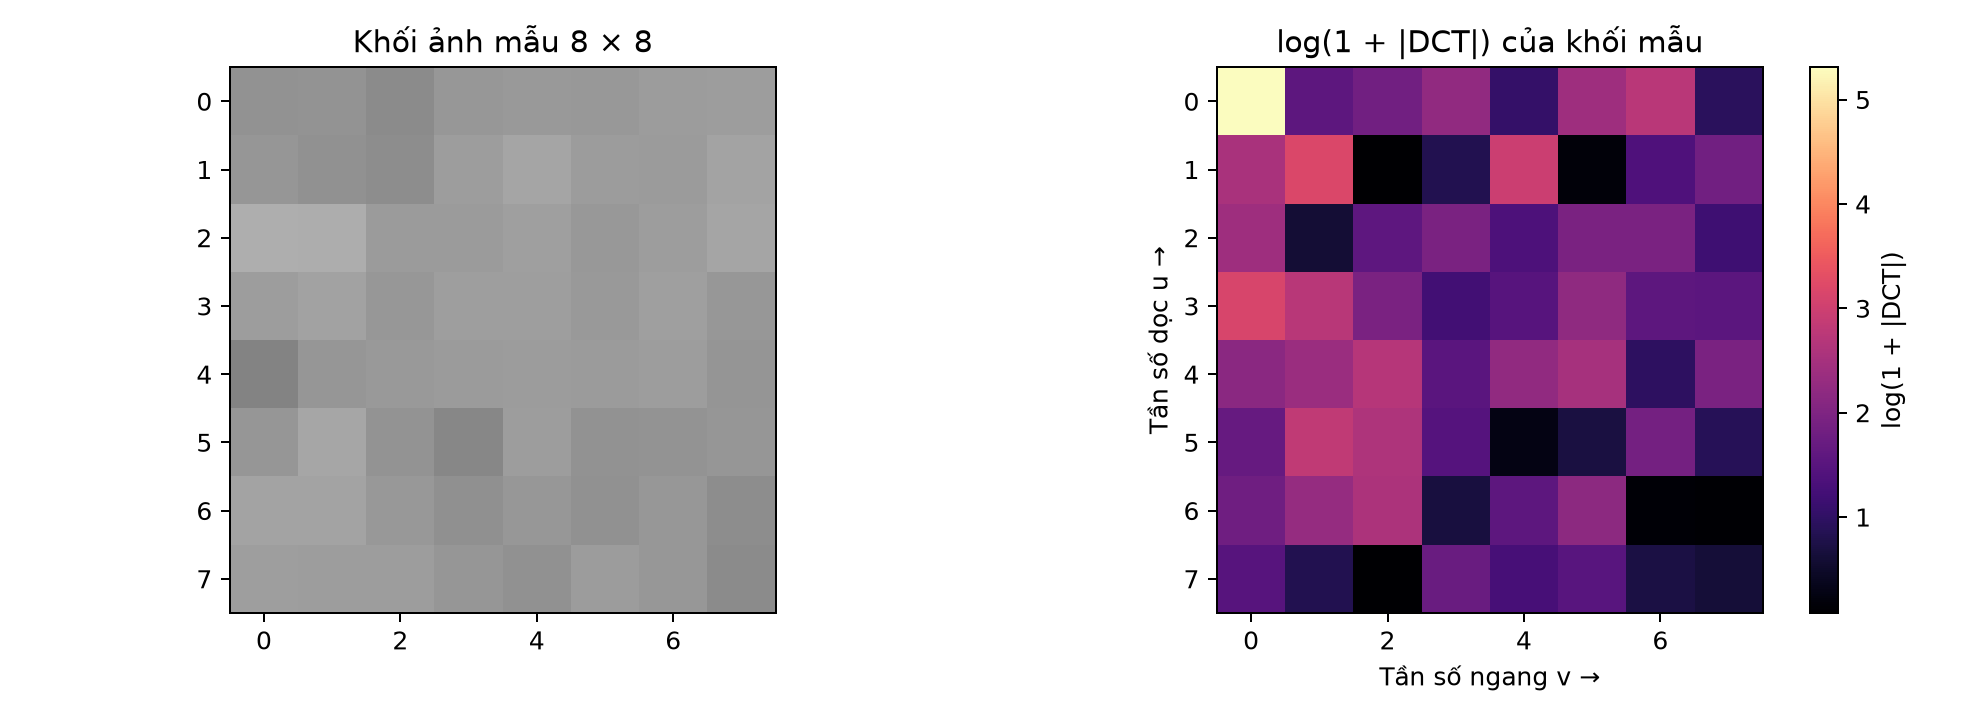
\includegraphics[width=\linewidth]{../code/ket_qua/cau2/dct.png}
\caption{Khối mẫu và độ lớn log(1 + |DCT|), kèm thang màu.}
\end{figure}
\FloatBarrier
DC = 201,375 có độ lớn vượt trội. Một số AC đáng kể gồm F[1,1] ≈ −22,75 và F[3,0] ≈ −22,10, nằm gần vùng tần số thấp. Nhiều hệ số phía dưới bên phải có độ lớn nhỏ, chẳng hạn F[6,6] ≈ 0,14 và F[7,7] ≈ −0,88. Biểu diễn log giúp nhìn thấy cả các AC nhỏ. Sự tập trung năng lượng phụ thuộc nội dung từng khối; khối có biên hoặc kết cấu mạnh vẫn có thể có AC tần số cao đáng kể.

\section{Câu 3 – Lượng tử hóa và dựng lại ảnh}
Tạo Q0[u,v] = 8 + 4 × (u + v), với u,v = 0,…,7. Với scale s > 0, tính Q = max(1, round(Q0 × s)) theo từng phần tử, lưu float32. Các hệ số được lượng tử hóa theo quantized = round(coefficients / Q), lưu int32. np.rint làm tròn về số chẵn gần nhất khi đúng nửa đơn vị.

Q tăng theo tần số, nên cùng độ lớn hệ số, các thành phần tần số cao dễ trở thành 0 hơn. Ở scale 1,0, bảng Q tăng từ 8 tại DC đến 64 tại góc dưới bên phải.

\subsection{Bảng Q tại scale = 1,0}
\begin{Verbatim}[fontsize=\scriptsize]
       8       12       16       20       24       28       32       36
      12       16       20       24       28       32       36       40
      16       20       24       28       32       36       40       44
      20       24       28       32       36       40       44       48
      24       28       32       36       40       44       48       52
      28       32       36       40       44       48       52       56
      32       36       40       44       48       52       56       60
      36       40       44       48       52       56       60       64
\end{Verbatim}
\subsection{Khối mẫu sau lượng tử hóa tại scale = 1,0}
\begin{Verbatim}[fontsize=\scriptsize]
      25        0        0        0        0        0        0        0
       1       -1        0        0        1        0        0        0
      -1        0        0        0        0        0        0        0
      -1       -1        0        0        0        0        0        0
       0        0        0        0        0        0        0        0
       0        0        0        0        0        0        0        0
       0        0        0        0        0        0        0        0
       0        0        0        0        0        0        0        0
\end{Verbatim}
DC được làm tròn từ 201,375 / 8 thành 25, giải lượng tử cho 200. Khối mẫu còn 7 hệ số khác 0 trên tổng 64 hệ số, tức 89,0625\% bằng 0. Đây là tỉ lệ riêng khối mẫu; tỉ lệ toàn ảnh tại scale 1,0 là khoảng 81,1\%.

\subsection{Quy trình mã hóa và chỉ tiêu đánh giá}
Quy trình: ảnh xám → chia khối/đệm → trừ 128 → DCT → lượng tử hóa → Zigzag → RLE → Huffman. Giải mã thực hiện các phép ngược, nhân Q, IDCT, cộng 128, ghép khối, cắt bỏ phần đệm, làm tròn và giới hạn về uint8.

MSE = tổng (I[y,x] − Î[y,x])² / (H × W), tính trên ảnh sau khi cắt phần đệm. Tỉ lệ hệ số 0 = số phần tử quantized bằng 0 / (N × 64). Số bit dữ liệu = len(bits), chỉ tính chuỗi Huffman; chưa tính bảng mã, Q và metadata. Các ảnh PNG lưu ra chỉ để quan sát ảnh dựng lại, không biểu diễn dung lượng tệp nén của bộ mô phỏng.

\clearpage
\subsection{Kết quả ảnh đầy đủ 240 × 416}
\begin{center}
\small\renewcommand{\arraystretch}{1.3}
\begin{tabular}{|p{3.30cm}|p{3.30cm}|p{3.30cm}|p{3.30cm}|}\hline
\textbf{Scale} & \textbf{MSE} & \textbf{Số bit dữ liệu} & \textbf{Hệ số bằng 0 (\%)} \\ \hline
0.5 & 12.3411 & 166,471 & 70.811 \\ \hline
1.0 & 30.4741 & 108,113 & 81.146 \\ \hline
3.0 & 97.4613 & 47,347 & 91.873 \\ \hline
\end{tabular}
\end{center}
\begin{figure}[!htbp]
\centering
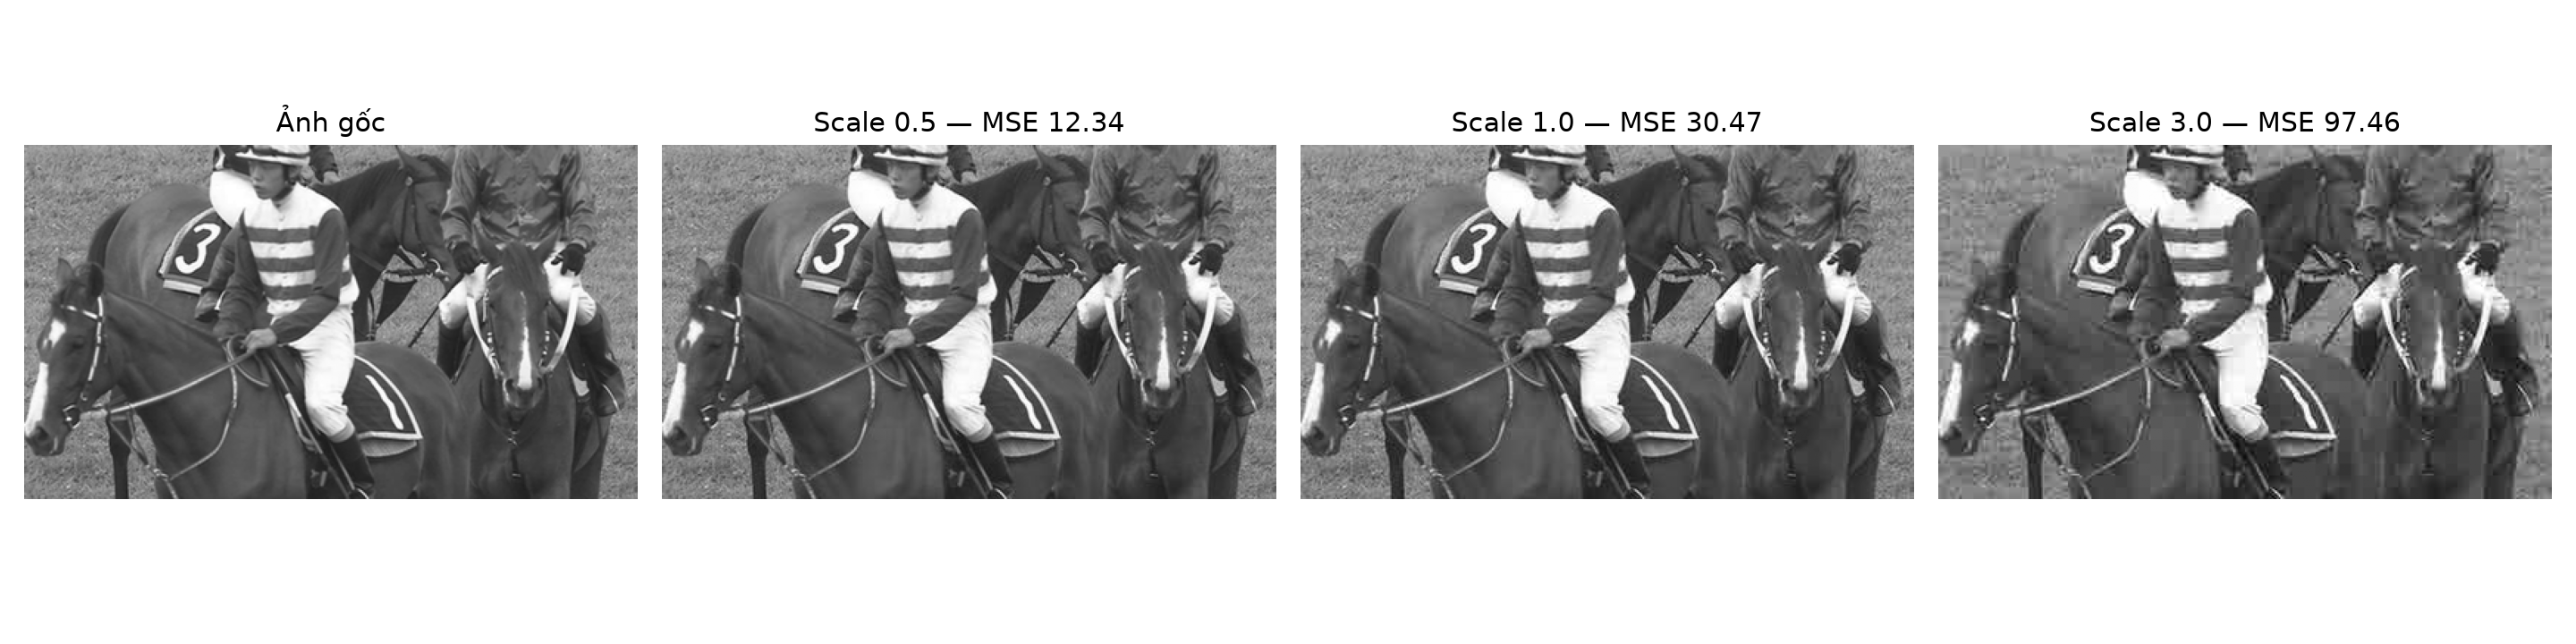
\includegraphics[width=\linewidth]{../code/ket_qua/cau3/anh_day_du_so_sanh.png}
\caption{Ảnh gốc và ảnh dựng lại tại scale 0,5; 1,0; 3,0 (cùng thang xám 0–255).}
\end{figure}
\FloatBarrier
Tại scale 0,5, ảnh giữ lại nhiều chi tiết hơn, MSE 12,34 và 70,8\% hệ số bằng 0. Tại scale 1,0, MSE tăng lên 30,47 và khoảng 81,1\% hệ số bằng 0. Tại scale 3,0, MSE đạt 97,46 và khoảng 91,9\% hệ số bằng 0; các chi tiết nhỏ và kết cấu bị làm mượt mạnh hơn.

Từ scale 0,5 đến 3,0, số bit giảm từ 166.471 xuống 47.347 (giảm khoảng 71,6\%), trong khi MSE tăng khoảng 7,9 lần. Scale 1,0 là mức trung gian trong ba cấu hình thử nghiệm; lựa chọn thực tế tùy yêu cầu chất lượng và dung lượng.

\clearpage
\subsection{Kết quả ảnh cắt 13 × 19}
\begin{center}
\small\renewcommand{\arraystretch}{1.3}
\begin{tabular}{|p{3.30cm}|p{3.30cm}|p{3.30cm}|p{3.30cm}|}\hline
\textbf{Scale} & \textbf{MSE} & \textbf{Số bit dữ liệu} & \textbf{Hệ số bằng 0 (\%)} \\ \hline
0.5 & 16.0445 & 480 & 73.958 \\ \hline
1.0 & 37.4413 & 245 & 86.198 \\ \hline
3.0 & 77.6235 & 63 & 96.354 \\ \hline
\end{tabular}
\end{center}
\begin{figure}[!htbp]
\centering
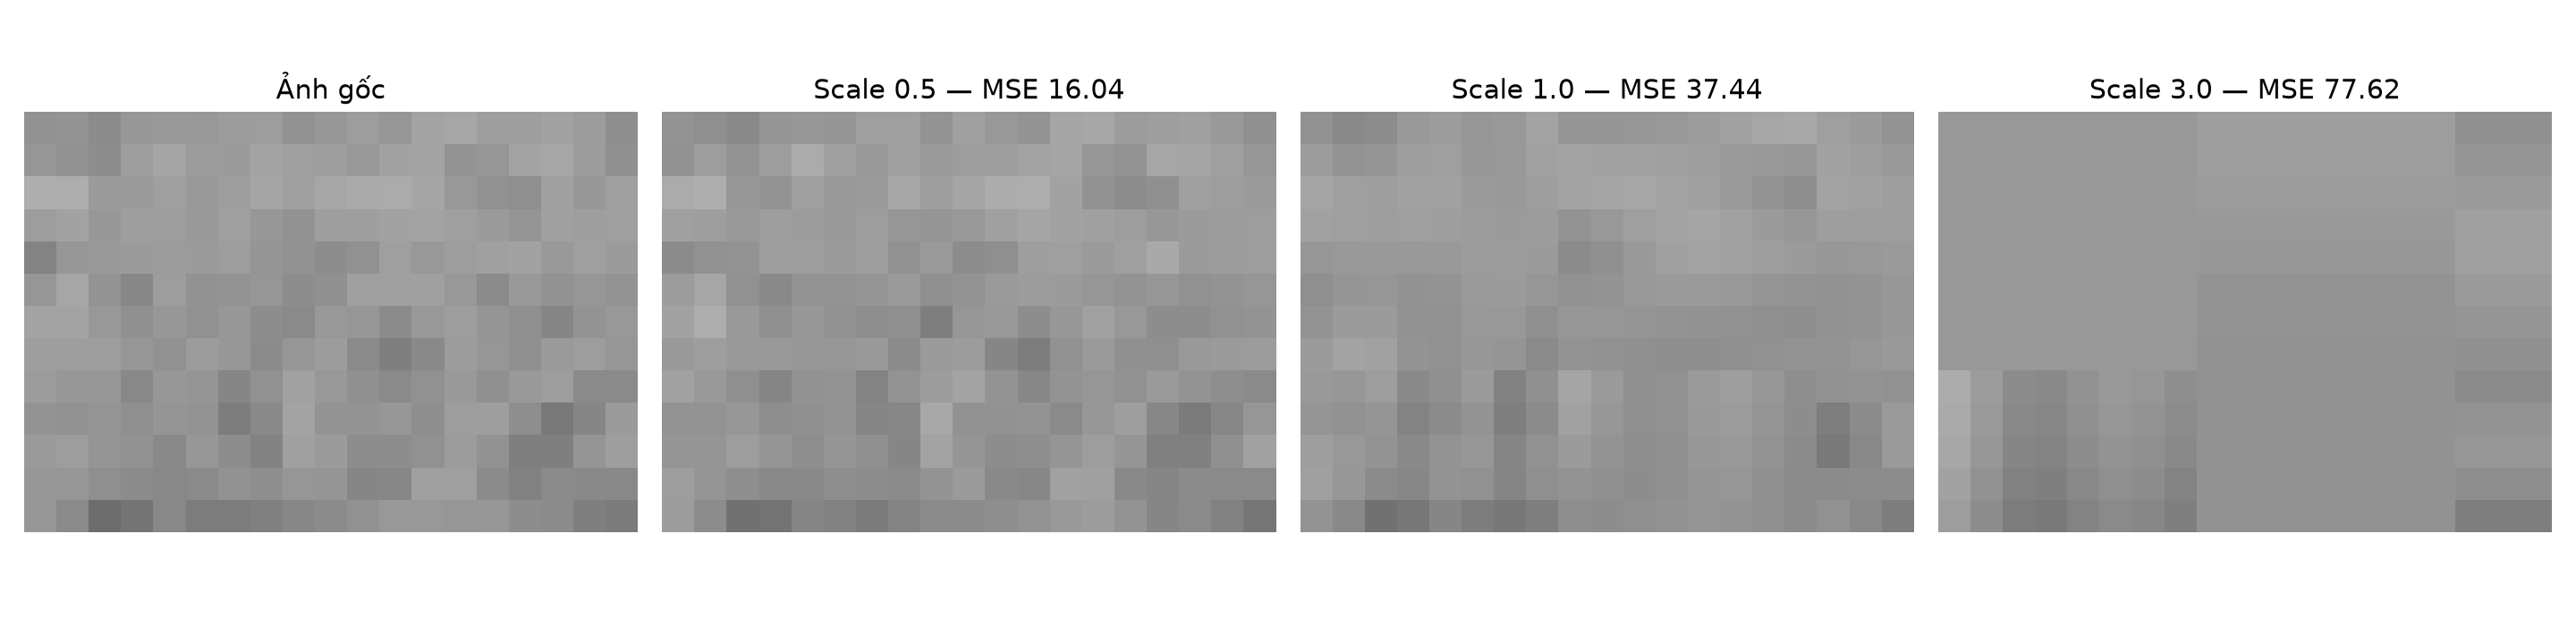
\includegraphics[width=\linewidth]{../code/ket_qua/cau3/anh_cat_13x19_so_sanh.png}
\caption{Ảnh gốc và ảnh dựng lại tại scale 0,5; 1,0; 3,0 (cùng thang xám 0–255).}
\end{figure}
\FloatBarrier
Ảnh cắt có 6 khối sau đệm thành 16 × 24. Ở cả ba mức, ảnh dựng lại đều có kích thước 13 × 19 và kiểu uint8. MSE được đo trên 247 điểm ảnh gốc, còn số bit và tỉ lệ hệ số 0 bao gồm 384 hệ số của các khối sau đệm. Vì vậy không so sánh trực tiếp số bit tuyệt đối của ảnh cắt với ảnh đầy đủ để kết luận hiệu quả nén.

MSE tăng từ 16,04 lên 77,62 khi tăng scale; số bit giảm từ 480 xuống 63. Tại scale 3,0, 96,4\% hệ số bằng 0. Ảnh cắt chứa ít nội dung và nhiều điểm ảnh đệm lặp lại nên có phân bố hệ số khác ảnh đầy đủ.

\subsection{Bước làm mất thông tin và kiểm tra tính đúng}
Lượng tử hóa là bước chủ yếu gây mất thông tin: nhiều giá trị DCT khác nhau cùng được làm tròn về một số nguyên, nên nhân lại Q không thể khôi phục chính xác hệ số ban đầu. DCT/IDCT chỉ có sai số tính toán số thực; thao tác làm tròn và cắt về [0,255] khi xuất ảnh cũng có thể bổ sung sai số. Zigzag, RLE và Huffman bảo toàn chính xác các hệ số nguyên đã lượng tử hóa.

Kiểm tra bổ sung đối chiếu hệ số trước mã hóa và sau giải mã bằng np.array\_equal; kiểm tra thứ tự ghép khối và giá trị đệm; kiểm tra DCT/IDCT trước lượng tử hóa. Với cả ảnh đầy đủ và ảnh cắt, ở cả ba scale, ảnh dựng lại có đúng kích thước và kiểu dữ liệu yêu cầu. Nhật ký kiểm tra được lưu tại bao\_cao/kiem\_tra.json.

\clearpage
\section{Kết luận và cách chạy lại}
Ba module đáp ứng chuỗi xử lí theo đề bài. Trên dữ liệu thực nghiệm, tăng scale làm tăng tỉ lệ hệ số bằng 0 và giảm độ dài chuỗi Huffman, đồng thời làm tăng MSE. Kiểm tra ảnh cắt xác nhận cơ chế đệm biên và cắt bỏ phần đệm khi giải mã hoạt động đúng. Bộ chương trình mô phỏng các bước nén ảnh xám, không tạo tệp JPEG chuẩn.

\begin{Verbatim}[fontsize=\scriptsize]
python -m pip install -r code/requirements.txt
python code/cau1_chia_khoi.py --no-show
python code/cau2_dct.py --no-show
python code/cau3_luong_tu_hoa.py --no-show
\end{Verbatim}
\section{Mã nguồn và tài liệu sử dụng}
Toàn bộ mã nguồn, ảnh đầu vào, thư viện cần cài đặt và kết quả thực nghiệm được lưu trong kho GitHub dưới đây. Ba module tự viết là cau1\_chia\_khoi.py, cau2\_dct.py và cau3\_luong\_tu\_hoa.py; jpeg\_support.py chứa mã hỗ trợ phần A của đề bài. README hướng dẫn cài đặt và chạy từng câu. Có thể tải toàn bộ kho bằng nút Code → Download ZIP hoặc dùng git clone.

\noindent\href{https://github.com/quansystems/compress_image}{\nolinkurl{https://github.com/quansystems/compress_image}}\par
\noindent\href{https://github.com/quansystems/compress_image/tree/main/code}{\nolinkurl{https://github.com/quansystems/compress_image/tree/main/code}}\par
Kho còn chứa verify\_results.py để kiểm tra dữ liệu và build\_report.py để tạo lại báo cáo. Nguồn LaTeX theo mẫu nằm trong BaoCaoTemplate/main.tex và BaoCaoTemplate/chapter/08\_NenAnh.tex.

Tài liệu sử dụng: Đề bài.pdf, Bài thực hành số 8, gồm yêu cầu Câu 1–3 và mã hỗ trợ phần A. Các bảng, ma trận và hình trong báo cáo được tạo từ ảnh đầu vào có sẵn trong thư mục code.
